\documentclass[11pt]{article}
\usepackage[pdftex]{graphicx}
\usepackage{Sweave}
\usepackage{amsmath}
\usepackage{amsfonts}
\addtolength{\textwidth}{1in}
\addtolength{\oddsidemargin}{-.5in}
\setlength{\evensidemargin}{\oddsidemargin}
%\setlength{\parskip}{0.5em}

\newcommand{\spp}{{\rm p}}
\newcommand{\match}{{\rm match}}
\newcommand{\st}{{\rm ST}}
\newcommand{\tttt}{{\rm TT}}
\newcommand{\tot}{{\rm TOT}}
\newcommand{\cat}{{\rm CT}}
\newcommand{\mcat}{{\rm MCT}}
\newcommand{\alter}{{\rm alter}}
\newcommand{\emse}{{\rm EMSE}}
\newcommand{\calt}{{\cal T}}
\newcommand{\est}{{\rm est}}
\newcommand{\calp}{{\Pi}}
\newcommand{\cals}{{\cal S}}

\newcommand{\mse}{{\rm MSE}}


\newcommand{\emset}{{\rm EMSE}_\tau}
\newcommand{\mset}{{\rm MSE}_\tau}
\newcommand{\emsem}{{\rm EMSE}_\mu}
\newcommand{\msem}{{\rm MSE}_\mu}
 
\newcommand{\msemw}{{\rm MSE}_{\mu,W}}
\newcommand{\control}{{\rm control}}
\newcommand{\treat}{{\rm treat}}
\newcommand{\alg}{{\rm alg}}
%\newcommand{\tree}{{\rm tree}}
\newcommand{\hemse}{\widehat{\rm EMSE}}
\newcommand{\oy}{\overline{Y}}
\newcommand{\ttt}{{\rm t}}
\newcommand{\cc}{{\rm c}}
\newcommand{\insample}{{\rm is}}
\newcommand{\outofsample}{{\rm os}}
\newcommand{\os}{{\rm os}}
\newcommand{\crit}{{\rm CRIT}}
\newcommand{\imgof}{{\rm imgof}}
\newcommand{\omgof}{{\rm omgof}}
\newcommand{\mgof}{{\rm mgof}}
\newcommand{\gof}{{\rm gof}}
\newcommand{\mx}{{\mathbb{X}}}
\newcommand{\train}{{\rm tr}}
\newcommand{\test}{{\rm te}}
\newcommand{\bx}{{\bf X}}
\newcommand{\ob}{\overline{b}}
\newcommand{\by}{{\bf Y}}
\newcommand{\bw}{{\bf W}}

\newcommand{\dif}{{\rm dif}}
\newcommand{\obs}{{\rm obs}}
\newcommand{\tree}{{\rm tree}}
\newcommand{\level}{{\rm level}}
\newcommand{\lasso}{{\rm lasso}}
%\newcommand{\match}{{\rm match}}
\newcommand{\transf}{{\rm transf}}
\newcommand{\ttrain}{{\rm train}}
\newcommand{\ttest}{{\rm test}}
\newcommand{\tcv}{{\rm cv}}
%\newcommand{\obs}{{\rm obs}}
\newcommand{\yin}{Y_i(0)}
\newcommand{\yie}{Y_i(1)}
\newcommand{\yio}{Y_i^\obs}
\newcommand{\mme}{\mathbb{E}}
\newcommand{\mmc}{\mathbb{C}}
\newcommand{\mmr}{\mathbb{R}}
\newcommand{\causal}{{\rm causal}}
\newcommand{\desc}{{\rm descr}}
\newcommand{\pop}{{\rm pop}}
\newcommand{\indep}{\perp\!\!\!\perp}







%\VignetteIndexEntry{Introduction to Rpart}
%\VignetteDepends{causalTree}
%\VignetteDepends{survival}
% Ross Ihaka suggestions
\DefineVerbatimEnvironment{Sinput}{Verbatim} {xleftmargin=2em}
\DefineVerbatimEnvironment{Soutput}{Verbatim}{xleftmargin=2em}
\DefineVerbatimEnvironment{Scode}{Verbatim}{xleftmargin=2em}
\fvset{listparameters={\setlength{\topsep}{0pt}}}
\renewenvironment{Schunk}{\vspace{\topsep}}{\vspace{\topsep}}


\newcommand{\myfig}[1]{\resizebox{\textwidth}{!}
                        {\includegraphics{#1.pdf}}}
\def\tree{\texttt{tree}}
\def\causalTree{\texttt{causalTree}}
\def\splus{S-Plus}
\newcommand{\Co}[1]{\texttt{#1}}

\title {An Introduction to Recursive Partitioning for Heterogeneous Causal Effects Estimation Using \texttt{causalTree} package}
\author{Susan Athey \\
        Guido Imbens\\
        Yanyang Kong}
\date{\today}

\begin{document}
\Sconcordance{concordance:briefintro.tex:briefintro.Rnw:%
1 252 1 1 2 1 0 1 4 3 0 1 1 4 0 1 2 82 1 1 5 4 0 1 1 28 0 1 1 4 0 1 2 1 %
1 1 2 1 0 2 1 4 0 1 2 3 1 1 2 1 0 2 2 1 3 1 0 2 2 1 9 7 0 3 2 4 0 1 2 3 %
1}

\maketitle
\tableofcontents

\section{Introduction}
This document is a brief introduction of \texttt{causalTree} package, which includes the \texttt{causalTree} function and the \texttt{honest.causalTree} function.  These implement the methods from \textit{Recursive Partitioning for Heterogeneous Causal Effects} \cite{athey2015machine}. \par 
The \texttt{causalTree} function builds a regression model and returns an \texttt{rpart} object, which is the object derived from \texttt{rpart} package, implementing many ideas in the CART (Classification and Regression Trees), written by Breiman, Friedman, Olshen and Stone \cite{Breiman83}. Like \texttt{rpart}, \texttt{causalTree} builds a binary regression tree model in two stages, but focuses on estimating heterogeneous treatment effects.  The function requires the user to specify a binary treatment variable in addition to the outcome variable and the
features that are usually passed to \texttt{rpart}.\par
Following \texttt{rpart}, in the first stage, the tree is grown from the root node based on a specified splitting rule. In each node, the data in a leaf will be split into two groups to best minimize the risk function. Next, in the left sub-node and right sub-node, the splitting routine will be applied separately and so on recursively until no improvements can made, or until some limits are reached (e.g. the routine will stop if it cannot make splits that have at least \texttt{minsize} of treated observations and \texttt{minsize} control observations in each terminal node.)
The risk for each node is calculated using a risk function associated with the splitting rule. \par
Unlike \texttt{rpart}, which estimates the average of the outcome variable in each leaf, \texttt{causalTree} estimates a treatment effect in each leaf by taking the difference
of the sample average of the treated group and the sample average of the control group within the leaf. The user selects one of several splitting rules for determining the optimal split
at each step.\par
The user also specifies a cross-validation method.  Cross-validation is implemented similar to \texttt{rpart}, where the cross-validation penalty parameter
penalizes the number of nodes in the tree.  The main difference arises in the cross-validation criterion, which is 
selected by the user.  The \texttt{cptable} of the \texttt{rpart} object includes the cross-validation error.   The user can choose to prune the tree using a specified cross-validation method, where  The leaves to be pruned are selected according to the risk function calculated while
the tree is built. \par
The \texttt{causalTree} package incorporates an additional function not included in \texttt{rpart}, which is honest re-estimation \texttt{honest.causalTree} of causal effects. Honest here means that we estimate causal effects in the leaves of a given tree on an independent estimation sample rather than the data used to build and cross-validate the tree.  The user first builds the tree
with \texttt{causalTree}, specifying the training data for building the tree, and then passes the tree object as well as the estimation sample data
into \texttt{honest.causalTree}, which replaces the leaf estimates from the input tree with new estimates in each leaf, calculated on the estimation sample.\par
To allow the user more control, there is another function, \texttt{estimate.causalTree}, that takes in an \texttt{rpart} object (which could have been estimated using the \texttt{rpart} package) and
replaces the leaf estimates with sample average treatment effects within each leaf, using a new dataset passed in by the user.  So it is possible to build a tree in either \texttt{causalTree}
or \texttt{rpart} using any one of a number of methods, and
then use \texttt{estimate.causalTree} to estimate treatment effects in each leaf on an arbitrary dataset. \par
The package has a few additional features not present in \texttt{rpart}.  One is that the \texttt{minsize} parameter requires that there are at least \texttt{minsize} treated and
\texttt{minsize} control observations in each leaf, so that a sample average treatment effect can be calculated. \par
Another feature is that we allow the user the option to restrict the set of potential split points considered,
and further, in the splitting process we rescale the covariate values within each leaf and each treatment group
in order to ensure that when moving
from one potential split point to the next, we move the same number of treatment and control observations from the right leaf to the left leaf.  \par
The rpart algorithm considers every value of every feature as a possible split point.
An obvious disadvantage of this approach is that computation time can grow prohibitively large in models with many observations
and features.  But there are some more subtle disadvantages as well. The first is that there will naturally be sampling variation
in calculating the risk function as we vary the possible split points. A problem akin to a multiple hypothesis testing problem arises:
since we are looking for the maximum value of an estimated criterion across a large number of possible split points,
as the number of split points tested grows, it becomes more and more likely that one of the splits for a given covariate appears to improve the fit criterion even if the true
value of the criterion would indicate that it is better not to split.  One way to mitigate both the computation time problem and
the multiple-testing problem is to consider only a limited number of split points. \par
A third problem is specific to considering treatment effect heterogeneity.  To see the problem, suppose that a covariate
strongly affects the mean of outcomes, but not treatment effects.  Within a leaf, some observations are treated and some
are control. If we consider every level of the covariate in the leaf as a possible split point, then shifting from one split point to the
next shifts a single observation from the right leaf to the left leaf.  This observation is in the treatment or the control group,
but not both; suppose it is in the treatment group.  If the covariate has a strong effect on the level of outcomes, the observation that is shifted will be likely have an
outcome more extreme than average. It will change the sample average of the treatment group, but not the control group, leading
to a large change in the estimated treatment effect difference.
We expect the estimated difference in treatment effects across the left and right leaves to fluctuate greatly with the split point in this scenario.  This
variability around the true mean difference in treatment effects occurs more often when covariates affect mean outcomes, and thus it
can lead the estimators to split too much on such covariates, and also to find spurious opportunities to split.\par
To address this problem, we incorporate the following modifications to the splitting rule.  We include a parameter \texttt{bucketNum}, 
the target number of observations per ``bucket.'' For each leaf, before testing possible
splits for a particular covariate, we order the observations by the covariate value in the treatment and control group separately.  Within each group, we place the observations into buckets with \texttt{bucketNum} observations per bucket.  If this results in less than \texttt{minsize} (another user-set parameter) buckets, then we use fewer observations
per bucket (to attain \texttt{minsize} buckets). If this results in more than \texttt{bucketMax} buckets, we use more observations per bucket to obtain \texttt{bucketMax} buckets.
We number the buckets, and considering potential splits by bucket number rather than the raw
values of the covariates.  This guarantees that when we shift from one split point to the next, we add both treatment and
control observations, leading to a smoother estimate of the goodness of fit function as a function of the split point.  After the
best bucket number to split on is selected, we translate that into a split point by averaging the maximum covariate value in
the corresponding treatment and control buckets.  


\section{Notation}
\begin{quote}
\begin{tabbing}
$X_i$ \qquad\qquad \= $i = 1, 2,..., N$ \qquad observed variables or feature matrix for observation $i$.\\
\\
$Y_i$ \> $i = 1, 2, ..., N$ \qquad observed outcome of observation $i$.\\
\\
$W_i$ \>$i = 1, 2, ..., N$ \qquad binary indicator for the treatment,\\
\>with $W_i = 0$ indicating that observation $i$ received the control treatment, \\
\>and $W_i = 1$ indicating that observation $i$ received the active treatment.\\
\\
$\cals$ \> a data sample drawn from data sample population, \\
\> $\cals^{\text{tr}}$ denotes a training sample,\\
\> $\cals^{\text{te}}$ denotes a test sample, \\
\> $\cals^{\text{est}}$ denotes an estimation sample.\\
\> $\cals_{\text{treat}}$ and $\cals_{\text{control}}$ denote the subsamples of treated and control units.\\
\\
$N$ 
\> $N^\train$ denotes the number of observations in training sample,\\
\> $N^\test$ denotes the number of observations in testing sample,\\
\> $N^\est$ denotes the number of observations in estimation sample.\\
\\
$\Pi$ \>  a partitioning tree $\calp=\{\ell_1,\ldots,\ell_{\#(\Pi)}\}$ with $\cup_{j=1}^{\#(\calp)} \ell_j=\mathbb{X}$ \\ 
\> corresponds to a partitioning of the feature space the feature space $\mathbb{X}$, with\\
\> $\#(\calp)$ the number of elements in the partition.\\
\\
$\ell(x; \calp)$ \> the leaf $\ell \in \calp$ such that $x \in \ell$.\\
\\

$\tau(\ell)$ \> $l = 1, 2, ..., k$ \qquad causal effect or treatment effect in leaf $\ell$. \\
\\
$p$ \> marginal treatment probability, $p = \text{pr}(W_i = 1)$. 

\end{tabbing}
\end{quote}



\section{Building Causal Trees}
\subsection{Splitting rules}
\texttt{causalTree} function offers four different splitting rules for user to choose. Each splitting rule corresponds to a specific risk function, and each split at a node aims to minimize the risk function. For each observation $(Y_i^{\text{obs}}, X_i, W_i)$, given a tree $\calp$, the population average outcome is 
\[\mu(w,x;\calp) \equiv \mme\left[\left. Y_i(w) \right| X_i\in\ell(x;\calp) \right], \]
and its average causal effect is 
\[\tau(x;\Pi) \equiv \mme\left[\left. Y_i(1)-Y_i(0) \right| X_i\in\ell(x;\calp) \right]. \]
the estimated outcome is
\[ \hat\mu(w,x;\cals,\calp) \equiv
\frac{1}{\#(\{i\in\cals_w:X_i\in\ell(x;\calp)\})}\sum_{i\in\cals_w:X_i\in\ell(x;\calp)} Y_i^\obs,\]
the estimated causal effect is the difference of treated mean and control mean in the leaf $l$ where it belongs,
\[ \hat\tau(x;\cals,\calp) \equiv \tau(\ell) =  \hat\mu(1,x;\cals,\calp)- \hat\mu(0,x;\cals,\calp).\]

\subsubsection{Transformed Outcome Trees (\textbf{TOT})}
We first define the transformed outcome as 
\[ Y_i^* = Y_i \cdot \frac{W_i - p}{p\cdot(1 - p)}\]
where $p = N_{\text{treat}} / N$ is the reatment probability, and
\[ Y^*_i = \begin{cases} 
     Y_i/p & W_i = 1 \\
      -Y_i/(1 - p) & W_i = 0
   \end{cases}
\]
In \textbf{TOT} splitting rule, the risk function is given by
\[\widehat{\mse}(\cals^\train, \cals^\train, \Pi) = \frac{1}{N^\train}\sum_{i\in\cals^\train}\left\{(Y^*_i - \hat{\tau}(X_i; \cals^\train, \calp))^2  - Y^{*2}_i\right\}\]

Note that the paper \cite{athey2015machine} envisions that treatment effects would be estimated by taking the mean of 
$Y_i^*$ within a leaf, but points out that this is inefficient because the treated fraction in a leaf may differ from the population
proportion due to sampling variation.  Thus, our package uses $\hat\tau$ instead.  The \texttt{rpart} package can be
used off-the-shelf (applied with $Y^*_i$ as the outcome) to implement the method precisely as described in \cite{athey2015machine}.

\subsubsection{Causal Trees (\textbf{CT})}
For the causal tree ``CT'' splitting rule, we have two versions, the adaptive verison, denoted as \textbf{CT-A}, and the honest version, \textbf{CT-H}. The user can select the honest version by setting \texttt{split.Honest = TRUE} in \texttt{causalTree} function. \\
For \textbf{CT-A}, we use $\widehat{\mse}_\tau(\cals^\train,\cals^\train,\calp)$ as the criterion (risk) function, and
\[-\widehat{\mse}_\tau(\cals^\train,\cals^\train,\calp) = \frac{1}{N^\train}\sum_{i\in\cals^\train} \hat\tau^2(X_i;\cals^\train,\calp).\]
\\
For \textbf{CT-H}, the honest version, the splitting criterion function is $\widehat{\emse}_\tau(\cals^\train, N^\est, \calp)$, and
\begin{align*}
-\widehat{\emse}_\tau(\cals^\train, N^\est, \calp) & = 
\frac{1}{N^\train}\sum_{i\in\cals^\train} \hat\tau^2(X_i;\cals^\train,\calp) \\
& -
\Bigl(\frac{1}{N^\train} + \frac{1}{N^\est}\Bigr)\cdot \sum_{\ell\in\calp}
\left( \frac{S^2_{\cals^\train_\treat}(\ell)}{p}+ \frac{S^2_{\cals^\train_\control}(\ell)}{1-p}\right).
\end{align*}
where $S^2_{\cals^\train_\control}(\ell)$ is the within-leaf variance on outcome $Y$ for $\cals^\train_\control$ in leaf $\ell$, and $S^2_{\cals^\train_\treat}(\ell)$ is the counter part for $\cals^\train_\treat$. $N^\est$ (the number of observations in re-estimation sample) is specified as \texttt{HonestSampleSize} in \texttt{causalTree} function, and the default value is $N^\train$.\\
In our package we incorporate an additional parameter \texttt{split.alpha} = $\alpha \in (0, 1)$ as a parameter to adjust the proportion of $\widehat{\mse}$ and the varaince term in $\widehat{\emse}$.
\begin{align*}
-\widehat{\emse}_\tau(\cals^\train, N^\est, \calp, \alpha) &= 
\alpha \cdot \frac{1}{N^\train}\sum_{i\in\cals^\train} \hat\tau^2(X_i;\cals^\train,\calp) \\
& - (1 - \alpha) \cdot
\Bigl(\frac{1}{N^\train} + \frac{1}{N^\est}\Bigr) \cdot \sum_{\ell\in\calp}
\left( \frac{S^2_{\cals^\train_\treat}(\ell)}{p}+ \frac{S^2_{\cals^\train_\control}(\ell)}{1-p}\right)
\end{align*}

\subsubsection{Fit-based Trees (\textbf{fit})}
In fit-based splitting rule, we decide at what value of the feature to split based on the goodness-of-fit of the outcome rather than the treatment effect. As \textbf{CT}, there are two versions of \textbf{fit}, namely adaptive version \textbf{fit-A} and honest version \textbf{fit-H}.\\
For \textbf{fit-A}, the objective risk function in splitting is 
\[\widehat{\mse}_{\mu, W}(\cals^\train,\cals^\train,\calp) =  \sum_{i\in\cals^\train} \left\{(Y_i-\hat\mu_w(W_i,X_i;\cals^\train,\calp))^2-Y^2_i\right\}\]
where $\hat\mu_w$ is the mean of outcome in treatment/control group.\\
\\
For \textbf{fit-H}, the honest version, the risk function is $\widehat{\emse}_{\mu, W}(\cals^\train, N^\est, \calp)$,
\begin{align*}
-\widehat{\emse}_{\mu, W}(\cals^\train, N^\est, \calp) & = 
\frac{1}{N^\train}\sum_{i\in\cals^\train} \hat\mu_w^2(W_i,X_i;\cals^\train,\calp) \\
& -
\Bigl(\frac{1}{N^\train} + \frac{1}{N^\est}\Bigr)\cdot \sum_{\ell\in\calp}
\left( S^2_{\cals^\train_\treat}(\ell)+ S^2_{\cals^\train_\control}(\ell)\right),
\end{align*}
where $S^2_{\cals^\train_\control}(\ell)$ is the within-leaf variance on outcome $Y$ for $\cals^\train_\control$ in leaf $\ell$, and $S^2_{\cals^\train_\treat}(\ell)$ is the counter part for $\cals^\train_\treat$. $N^\est$ (the number of observations in re-estimation sample) is specified as \texttt{HonestSampleSize} in \texttt{causalTree} function, and the default value is $N^\train$.\\
Also like \textbf{CT}, we have adjusted honest verison for $\widehat{\emse}_{\mu, W}$ using \texttt{split.alpha},
\begin{align*}
-\widehat{\emse}_{\mu, W}(\cals^\train, N^\est,\calp, \alpha) & = 
\alpha \cdot \frac{1}{N^\train}\sum_{i\in\cals^\train} \hat\mu_w^2(W_i,X_i;\cals^\train,\calp) \\
& - (1 - \alpha) \cdot
\Bigl(\frac{1}{N^\train} + \frac{1}{N^\est}\Bigr)\cdot \sum_{\ell\in\calp}
\left( S^2_{\cals^\train_\treat}(\ell)+ S^2_{\cals^\train_\control}(\ell)\right),
\end{align*}

\subsubsection{Squared T-statistic Trees (\textbf{tstats})}
In squared t-statistic (``tstats'') trees, we consider the splits with the largest value for square of the t-statistic for testing the null hypothesis that the average treatment effect is the same in the two potential leaves. Denote the left leaf as L and right leaf as R, the square of the t-statistic is 
\[ T^2 \equiv \frac{((\oy_{L1}-\oy_{L0})-
(\oy_{R1}-\oy_{R0})
)^2}{S_{L1}^2/N_{L1}+ S_{L0}^2/N_{L0}+S_{R1}^2/N_{R1}+S_{R0}^2/N_{R0}},\]
where $S_{\ell,w}^2$ is the conditional within treatment group sample variance given the split.  Unlike the mean-squared error criteria, the ``tstats'' criterion does not neatly 
decompose into a risk for each observation; thus, it is not obvious what criterion to use for determining which leaves to prune first when pruning the tree.  Our package uses
the ``CT-H'' criterion function. 
\subsection{Discrete splitting}
As motivated in the introduction, the package includes the option to consider a discrete set of splitting points. To use discrete splitting, the user should set \texttt{split.Bucket = TRUE} and specify\texttt{bucketNum}, \texttt{bucketMax}. The default value of \texttt{bucketNum = 5} and \texttt{bucketMax = 100}.\par
In discrete splitting, the samples in a node will be sorted by value of a feature separately for the treated and control groups, and then observations will be partitioned in to buckets. The number of buckets is determined as $\text{min}(\texttt{bucketMax},\text{max}(n_{min}/\texttt{bucketNum},\texttt{minsize}))$ observations, where $n_{min}$ is the minimum of the 
number of treated observations and the number of control observations in the leaf to be split. Then one bucket will be treated as a whole and assigned into left branch or right branch. 

\subsection{Example}
The data we use in this example is a simulated data set called \texttt{simulation.1} built in \texttt{causalTree} package. \par
In this model, we choose \textbf{TOT} as splitting rule and \textbf{fit} as cross validation method by setting \texttt{split.Rule = "TOT"} and \texttt{cv.option = "fit"}. The propensity score (treatment probability) is set as \texttt{propensity = 0.5} for \textbf{TOT} splitting rule. We also use the discrete splitting option by setting \texttt{split.Bucket = T}.
\begin{Schunk}
\begin{Sinput}
> library(causalTree)
> tree <- causalTree(y ~ x1 + x2 + x3 + x4, data = simulation.1, 
+                   treatment = simulation.1$treatment, split.Rule = "TOT",
+                   cv.option = "fit", cv.Honest = F, split.Bucket = T, 
+                   xval = 10, cv.alpha = 0.5, propensity = 0.5)
> rpart.plot(tree)
\end{Sinput}
\end{Schunk}
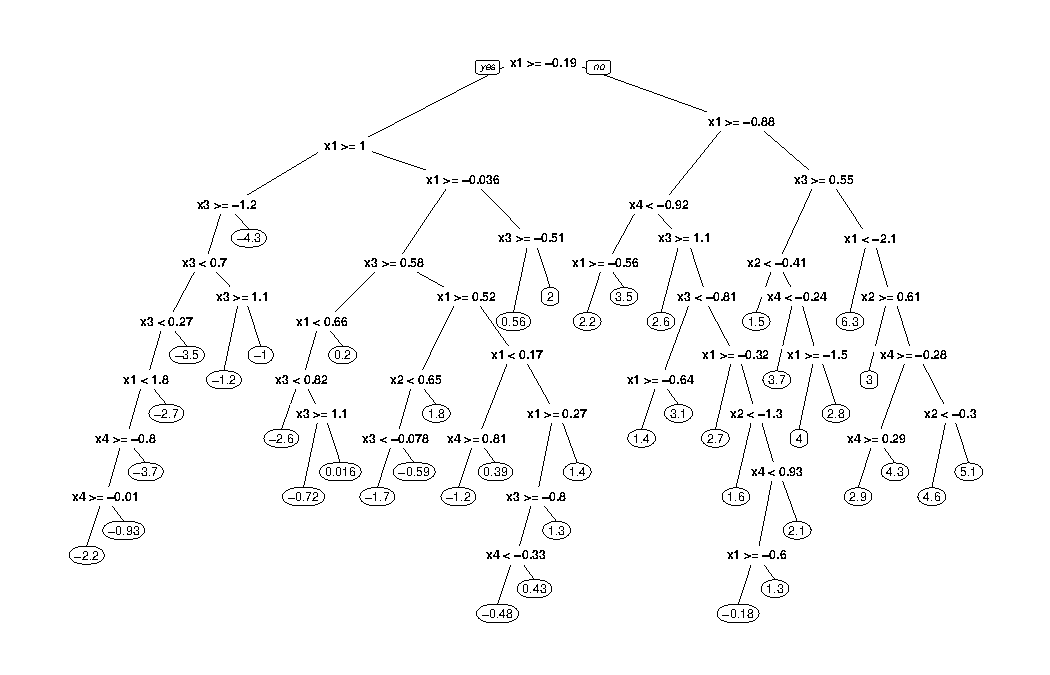
\includegraphics{briefintro-example1}

From the plot we can see, without pruning, the tree we get is quite large. The following section will describe different cross validation methods to prune the tree.

\section{Cross Validation and Pruning}
Following \texttt{rpart}, we will build cross validation trees to select a complexity parameter corresponding to the minimum cross validaiton error used for pruning. Different from \texttt{rpart}, in cross validation, we can choose different evaluation criteria to calculate the error.
\subsection{Cross validation options}
We offer four criteria for cross validation, \textbf{TOT}, \textbf{CT}, \textbf{fit} and \textbf{matching}. Each criterion corresponds to an evaluation function for computing the cross-validation error. When building trees in the cross-validation process, we use the original splitting rule (specified by \texttt{split.Rule}), but the cross validation error evaluation function is determined by \texttt{cv.option}.
\subsubsection{TOT}
When \texttt{cv.option}=\textbf{TOT}, the evaluation function is
\[\widehat{\mse}(\cals^{\train, \tcv}, \cals^{\train, \train}, \Pi) = \frac{1}{N^{\train, \tcv}}\sum_{i\in\cals^{\train, \tcv}}\left\{(Y^*_i - \hat{\tau}(X_i; \cals^{\train, \train}, \calp))^2  - Y^{*2}_i\right\}
\]
where $\cals^{\train, \train}$ is part of training sample used for building cross validaiton trees and $\cals^{\train, \tcv}$ is the other part of training sample (referred to here as the validation sample) used for predicting and calculating the error, and $N^{\train, \tcv}$ is the number of observations in $\cals^{\train, \tcv}$.  There is no ``honest'' option for this method.

\subsubsection{CT}
When \texttt{cv.option}=\textbf{CT}, there are two versions, adaptive and honest. We denote them as \textbf{CT-A} and \textbf{CT-H}. \\
For the \textbf{CT-A} cross validation method, the evaluation funciton is
\begin{align*}
\widehat{\mse}_\tau(\cals^{\train, \tcv},\cals^{\train, \train},\calp) =&
-\frac{2}{N^{\train, \tcv}}\sum_{i\in\cals^{\train, \tcv}}\hat\tau(X_i;\cals^{\train, \tcv},\calp)\hat\tau(X_i;\cals^{\train, \train},\calp)\\
& + \frac{1}{N^{\train, \tcv}}\sum_{i\in\cals^{\train, \tcv}}\hat\tau^2(
X_i;\cals^{\train, \train},\calp),
\end{align*}
where $\hat\tau(X_i;\cals^{\train, \tcv},\calp)$ is the treatment effect calculated in the validation sample and $\hat\tau(X_i;\cals^{\train, \train},\calp)$ is the treatment effect in the training component $\cals^{\train, \train}$.\\
For \textbf{CT-H} cross validation method, the evaluation function is $\widehat{\emse}_\tau(\cals^{\train, \tcv}, N^\est, \calp)$, and 
\begin{align*}
-\widehat{\emse}_\tau(\cals^{\train, \tcv}, N^\est, \calp) & = 
\frac{1}{N^{\train, \tcv}}\sum_{i\in\cals^{\train, \tcv}} \hat\tau^2(X_i;\cals^{\train, \tcv},\calp) \\
& -
\Bigl(\frac{1}{N^{\train, \tcv}} + \frac{1}{N^\est}\Bigr)\cdot \sum_{\ell\in\calp}
\left( \frac{S^2_{\cals^{\train, \tcv}_\treat}(\ell)}{p}+ \frac{S^2_{\cals^{\train, \tcv}_\control}(\ell)}{1-p}\right).
\end{align*}
Like its splitting method, we also incorporate an additional factor \texttt{cv.alpha} for adjustment of two terms in the formula,
\begin{align*}
-\widehat{\emse}_\tau(\cals^{\train, \tcv}, N^\est, \calp, \alpha) & = 
\alpha \cdot \frac{1}{N^{\train, \tcv}}\sum_{i\in\cals^{\train, \tcv}} \hat\tau^2(X_i;\cals^{\train, \tcv},\calp) \\
& - (1 - \alpha) \cdot
\Bigl(\frac{1}{N^{\train, \tcv}} + \frac{1}{N^\est}\Bigr)\cdot \sum_{\ell\in\calp}
\left( \frac{S^2_{\cals^{\train, \tcv}_\treat}(\ell)}{p}+ \frac{S^2_{\cals^{\train, \tcv}_\control}(\ell)}{1-p}\right).
\end{align*}


\subsubsection{fit}
Like its splitting counterpart, \textbf{fit} cross validation criterion also has adaptive version \textbf{fit-A} and honest version \textbf{fit-H} to evaluate the model.\\
For \textbf{fit-A} criterion, the evaluation risk function is  
\[\widehat{\mse}_{\mu, W}(\cals^{\train, \tcv},\cals^{\train, \train},\calp) =  \sum_{i\in\cals^{\train, \tcv}} \left\{(Y_i-\hat\mu_w(W_i,X_i;\cals^{\train, \train},\calp))^2-Y^2_i\right\}\]
where $\hat\mu_w(W_i,X_i;\cals^{\train, \train},\calp)$ is the mean of outcome in treatment/control group of the built cross validation tree where validation sample $(X_i, Y_i, W_i) \in \cals^{\train, \tcv}$ finally be assigned.\\
\\
For \textbf{fit-H} criterion, the evaluation function is $\widehat{\emse}_{\mu, W}(\cals^{\train, \tcv}, N^\est, \calp)$,
\begin{align*}
-\widehat{\emse}_{\mu, W}(\cals^{\train, \tcv}, N^\est, \calp) & = 
\frac{1}{N^{\train, \tcv}}\sum_{i\in\cals^{\train, \tcv}} \hat\mu_w^2(W_i,X_i;\cals^{\train, \tcv},\calp) \\
& -
\Bigl(\frac{1}{N^{\train, \tcv}} + \frac{1}{N^\est}\Bigr)\cdot \sum_{\ell\in\calp}
\left( S^2_{\cals^{\train, \tcv}_\treat}(\ell)+ S^2_{\cals^{\train, \tcv}_\control}(\ell)\right),
\end{align*}
In contrast to the adaptive version, $\hat\mu_w(W_i,X_i;\cals^{\train, \tcv},\calp)$ is the mean of outcome derived from the validation group.\\
Also we incorporate \texttt{cv.alpha} for adjustment in \textbf{CT-H} evaluation function,
\begin{align*}
-\widehat{\emse}_{\mu, W}(\cals^{\train, \tcv}, N^\est, \calp, \alpha) & = 
\alpha \cdot \frac{1}{N^{\train, \tcv}}\sum_{i\in\cals^{\train, \tcv}} \hat\mu_w^2(W_i,X_i;\cals^{\train, \tcv},\calp) \\
& - (1 - \alpha) \cdot
\Bigl(\frac{1}{N^{\train, \tcv}} + \frac{1}{N^\est}\Bigr)\cdot \sum_{\ell\in\calp}
\left( S^2_{\cals^{\train, \tcv}_\treat}(\ell)+ S^2_{\cals^{\train, \tcv}_\control}(\ell)\right).
\end{align*}


\subsubsection{matching}
In \textbf{matching} method, we first define $n(W_i, X_i; \cals)$ to be the nearest neighbor of $(X_i, Y_i, W_i)$ in feature space with opposite $W$.\\
To be more specific, let $j = n(W_i, X_i; \cals)$, then 
\begin{align*}
 & (X_j, Y_j, W_j) \in \cals, \\
 & W_j = 1 - W_i,\\
 & d_X((X_j, Y_j, W_j), (X_i, Y_i, W_i)) = \min_{\substack{
 (X_k, Y_k, W_k) \in \cals,\\ W_k = 1 - W_i }} d_X((X_k, Y_k, W_k), (X_i, Y_i, W_i)).
\end{align*}
Then we can define the \textbf{matching} estimator of treatment effect as
\[\tau^*(X_i, W_i; \cals) \equiv (2W_i - 1) (Y_i - Y_{n(W_i, X_i; \cals)})\]
The evaluation risk function in \textbf{matching} method is
\[
\widehat\mse_{\tau}(\cals^{\train, \tcv}, \cals^{\train, \train}, \calp) = \sum_{i \in \cals^{\train, \tcv}}\left(\tau^*(X_i, W_i; \cals) - \frac{\hat{\tau}(X_i; \cals^{\train, \train}, \calp) + \hat{\tau}(X_{n(W_i, X_i; \cals^{\train, \tcv})}; \cals^{\train, \train}, \calp )}{2}\right)^2
\]
\subsection{Example}

In the following example, we choose honest splitting rule as \textbf{CT-H} (\texttt{split.Rule ="CT"}, \texttt{split.Honest = T}), and cross validation method as \textbf{matching} (\texttt{cv.option = "matching"} and \texttt{cv.Honest = F}). We set 10 folds cross validation (\texttt{xval = 10}) and print out the \texttt{cptable} to check out the complexity parameter (\texttt{cp}) and normalized cross validation error (\texttt{xerror}).
\begin{Schunk}
\begin{Sinput}
> tree <- causalTree(y ~ x1 + x2 + x3 + x4, data = simulation.1, 
+                   treatment = simulation.1$treatment, split.Rule = "CT",
+                   split.Honest = T, cv.option = "matching", cv.Honest = F, 
+                   split.Bucket = F, xval = 10)
> tree$cptable
\end{Sinput}
\begin{Soutput}
             CP nsplit rel error    xerror        xstd
1  1.145837e-02      0 1.0000000 1.0000000 0.002544452
2  1.941622e-03      1 0.9885416 0.5141833 0.001487195
3  1.862875e-03      2 0.9866000 0.5129707 0.001411806
4  1.031403e-03      3 0.9847371 0.4762972 0.001260437
5  7.763028e-04      5 0.9826743 0.4471484 0.001116234
6  5.128562e-04      8 0.9803454 0.4203597 0.001078958
7  4.327552e-04     10 0.9793197 0.4197124 0.001068104
8  3.525900e-04     11 0.9788870 0.4226628 0.001067524
9  3.052253e-04     13 0.9781818 0.4302321 0.001095403
10 2.632508e-04     14 0.9778766 0.4621311 0.001207203
11 2.198657e-04     16 0.9773500 0.4899981 0.001275376
12 1.945478e-04     17 0.9771302 0.5248392 0.001358469
13 1.887622e-04     18 0.9769356 0.5248630 0.001364536
14 1.792430e-04     19 0.9767469 0.5342639 0.001361384
15 1.677139e-04     20 0.9765676 0.5296446 0.001341866
16 1.366938e-04     25 0.9756676 0.5243033 0.001334980
17 1.111979e-04     28 0.9752575 0.5361940 0.001354982
18 1.096178e-04     32 0.9747981 0.5363380 0.001346708
19 1.002128e-04     36 0.9743597 0.5360979 0.001347304
20 7.376079e-05     37 0.9742595 0.5436176 0.001345552
21 4.858865e-05     38 0.9741857 0.5597567 0.001375235
22 2.870558e-05     39 0.9741371 0.5652205 0.001389057
23 0.000000e+00     40 0.9741084 0.5682949 0.001396325
\end{Soutput}
\begin{Sinput}
> rpart.plot(tree)
\end{Sinput}
\end{Schunk}
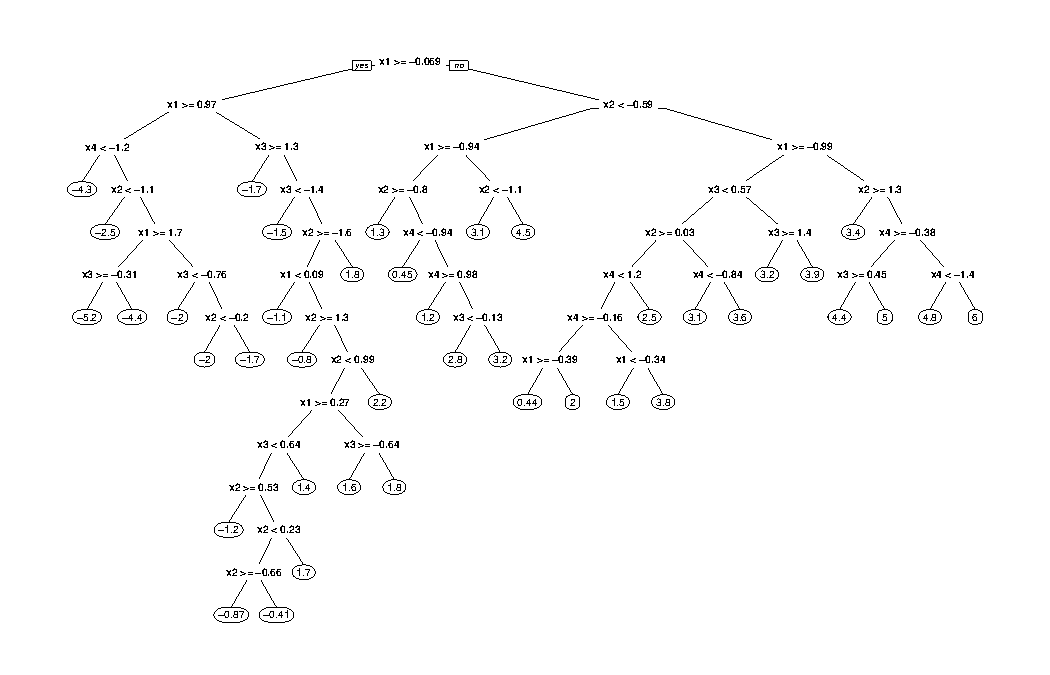
\includegraphics{briefintro-example2}
\\
The built tree in the plot is large and deep. Like \texttt{rpart}, we choose the complexity paramter \texttt{opcp} corresponding to the minimum cross validation error (\texttt{xerror}) in \texttt{tree\$cptable}, and use the function \texttt{prune()} to trim the tree: 
\begin{Schunk}
\begin{Sinput}
> opcp <- tree$cptable[, 1][which.min(tree$cptable[,4])]
> optree <- prune(tree, cp = opcp)
> rpart.plot(optree)
\end{Sinput}
\end{Schunk}
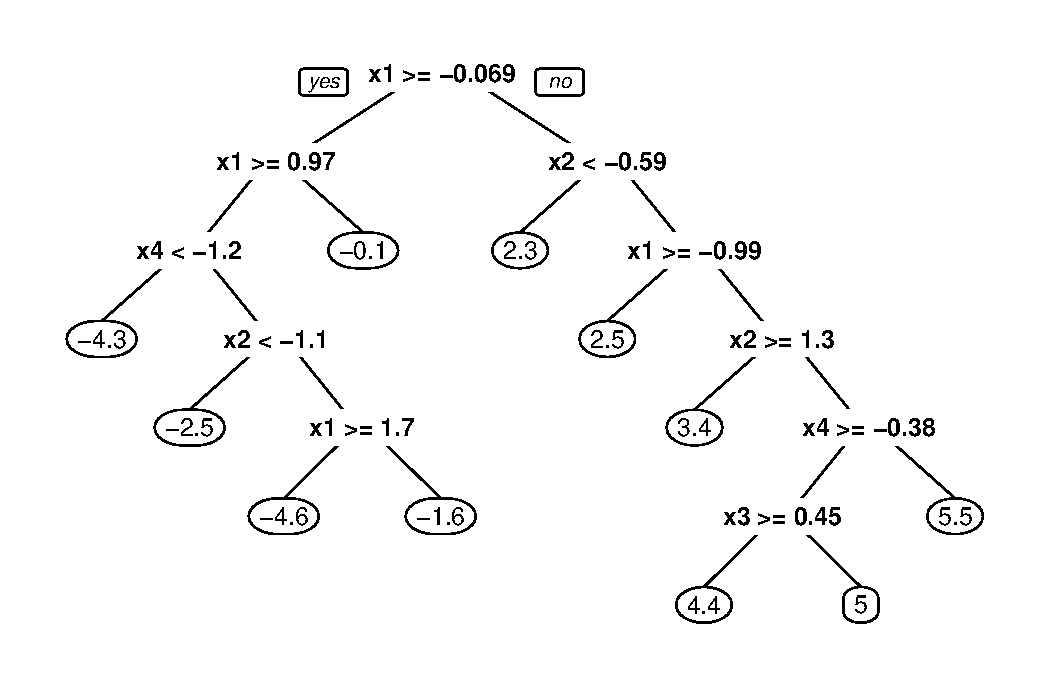
\includegraphics{briefintro-prune}
\section{Honest Estimation}
In addtion to \texttt{causalTree}, we also support one-step honest re-estimation in function \texttt{honest.causalTree}. It can fit a \texttt{causalTree} model and get honest estimation results with tree structre built on training sample (including cross validation) and leaf treatment effect estimates taken from estimation sample.

\subsection{Example}
\begin{Schunk}
\begin{Sinput}
> n <- nrow(simulation.1)
> trIdx <- which(simulation.1$treatment == 1)
> conIdx <- which(simulation.1$treatment == 0)
> train_idx <- c(sample(trIdx, length(trIdx) / 2), 
+                sample(conIdx, length(conIdx) / 2))
> train_data <- simulation.1[train_idx, ]
> est_data <- simulation.1[-train_idx, ]
> honestTree <- honest.causalTree(y ~ x1 + x2 + x3 + x4, data = train_data,
+                                 treatment = train_data$treatment, 
+                                 est_data = est_data, 
+                                 est_treatment = est_data$treatment, 
+                                 split.Rule = "CT", split.Honest = T, 
+                                 HonestSampleSize = nrow(est_data), 
+                                 split.Bucket = T, cv.option = "fit",
+                                 cv.Honest = F)
> opcp <-  honestTree$cptable[,1][which.min(honestTree$cptable[,4])]
> opTree <- prune(honestTree, opcp)
> rpart.plot(opTree)
\end{Sinput}
\end{Schunk}
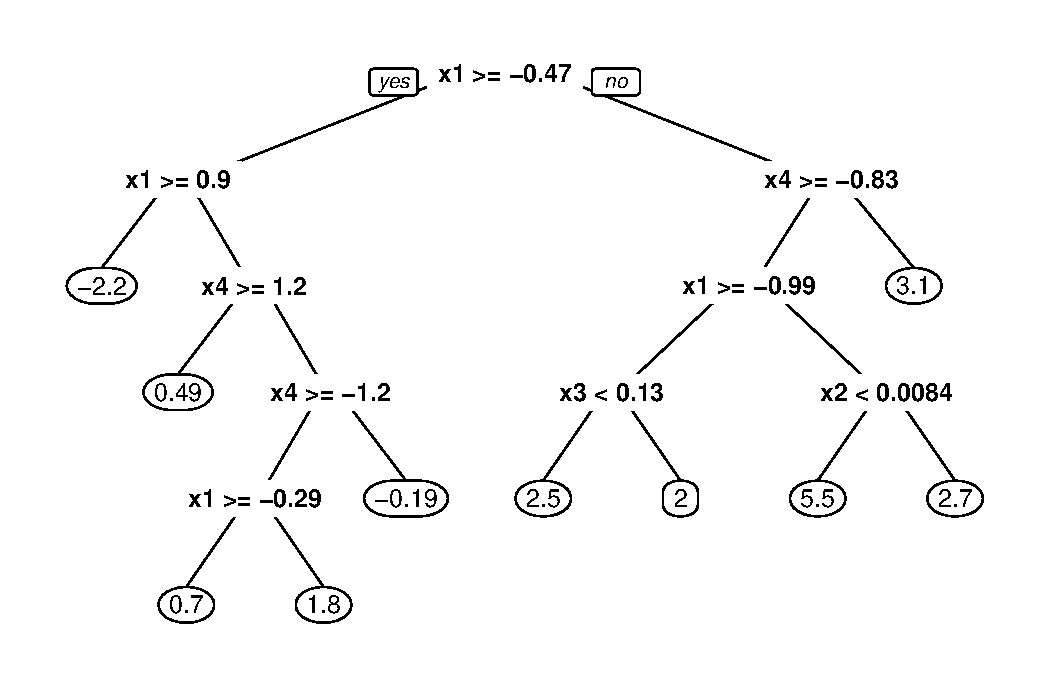
\includegraphics{briefintro-example3}

\bibliographystyle{plain}
\bibliography{refer}
\end{document}
